\section{Loan Application Process}
\label{sec:loan-app-process}

\subsection{General Information}
\label{sec:loan-app-information}

In this section, methodology proposed in this thesis study will be applied on the \textit{Loan Application Process} dataset \cite{loan-app-data} and evaluation results will be presented. Statistical information about this dataset is presented in Table~\ref{table:loan-app-process-summary} to provide an insight about this dataset.
%\caption{Statistical summary of Loan Application Process Dataset}
%\label{table:loan-app-process-summary}
\begin{table}[]
\centering
\caption{Statistical summary of Loan Application Process dataset}
\label{table:loan-app-process-summary}
\begin{tabular}{@{}lccc@{}}
\toprule
                  & {\bf Cases} & {\bf Events} & {\bf Percentage} \\ \midrule
{\bf Variant \#1} & 100         & 590          & 24 \%            \\ \midrule
{\bf Variant \#2} & 70          & 420          & 17 \%            \\ \midrule
{\bf Variant \#3} & 200         & 800          & 33 \%            \\ \midrule
{\bf Variant \#4} & 105         & 630          & 26 \%            \\ \midrule
{\bf Total}       & {\bf 475}   & {\bf 2440}   & {\bf }           \\ \bottomrule
\end{tabular}
\end{table}

As shown in Table~\ref{table:loan-app-process-summary}, total of 475 cases and 2440 events included in this dataset with a fairly even distribution between variants. In the following section, these variants will be used as organizational logs and the methodology presented in this thesis study will be applied.

\subsection{Methodology Stages}
\label{sec:loan-app-methodology}
In \textit{Process Model Mining} stage, variants of the dataset are used as organizational event logs and they are used to mine process models. Since dataset is synthetically generated, noise threshold in \textit{Inductive Miner} is set to 0 and perfect log fitness is ensured. Appropriateness and fitness evaluation metrics are summarized in Table~\ref{table:loan-app-process-process-model-mining} and it can be seen that each event log is successful in terms of representing reality and being appropriate as a process model. Especially for the variants other than Variant \#1, there is a perfect fitness and appropriateness as it is expected from a  synthetically generated dataset without noise. In addition, process models for each event log is visualized in Figure~\ref{fig:loan-application-process-models}.
%\caption{Process Model Mining Evaluation of Loan Application Process Dataset}
%\label{table:loan-app-process-process-model-mining}
\begin{table}[]
\centering
\caption{Process Model Mining Evaluation of Loan Application Process Dataset}
\label{table:loan-app-process-process-model-mining}
\begin{tabular}{lcccc}
\hline
 & {\bf Fitness} & {\bf \begin{tabular}[c]{@{}c@{}}Structural\\Appropriateness\end{tabular}} & {\bf \begin{tabular}[c]{@{}c@{}}Behavioral\\Appropriateness\end{tabular}} & {\bf \begin{tabular}[c]{@{}c@{}}Average\\Appropriateness\end{tabular}} \\ \hline
{\bf Variant \#1} & 100 \% & 70 \% & 98.5 \% & 84.2 \% \\ \hline
{\bf Variant \#2} & 100 \% & 100 \% & 100 \% & 100 \% \\ \hline
{\bf Variant \#3} & 100 \% & 100 \% & 100 \% & 100 \% \\ \hline
{\bf Variant \#4} & 100 \% & 100 \% & 98.2 \% & 99.1 \% \\ \hline
{\bf Average} & {\bf 100 \%} & {\bf 92.5 \%} & {\bf 99.7 \%} & {\bf 96.06 \%} \\ \hline
\end{tabular}
\end{table}
\begin{figure}
\centering
  \begin{subfigure}{.4\textwidth}
    \centering
    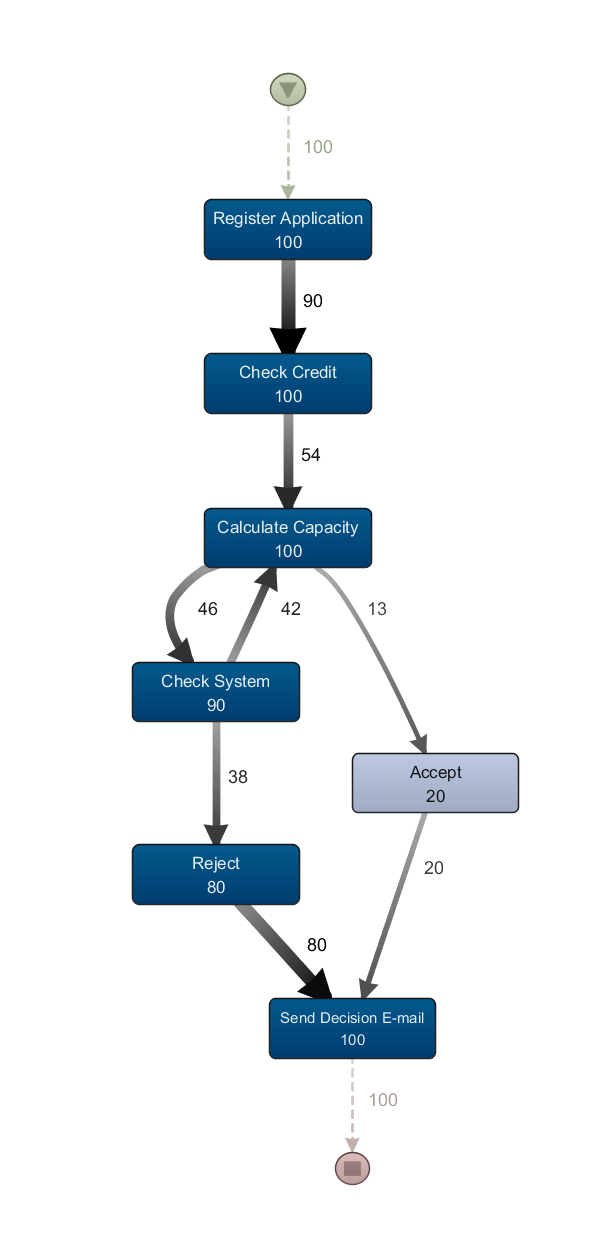
\includegraphics[width=.8\linewidth]{5_results_discussions/loan-application-process/ETM_Configuration1}
    \caption{Variant \#1}
    \label{fig:loan-application-process-models-1}
  \end{subfigure}%
  \begin{subfigure}{.4\textwidth}
    \centering
    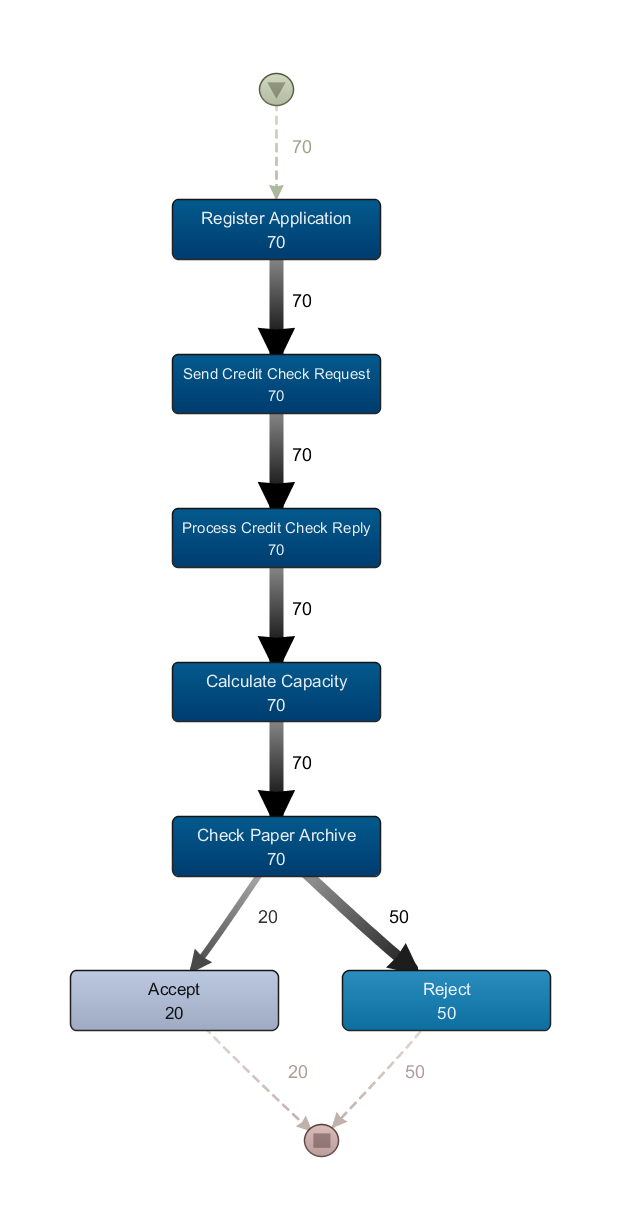
\includegraphics[width=.8\linewidth]{5_results_discussions/loan-application-process/ETM_Configuration2}
    \caption{Variant \#2}
    \label{fig:loan-application-process-models-2}
  \end{subfigure} \\
  \begin{subfigure}{.4\textwidth}
    \centering
    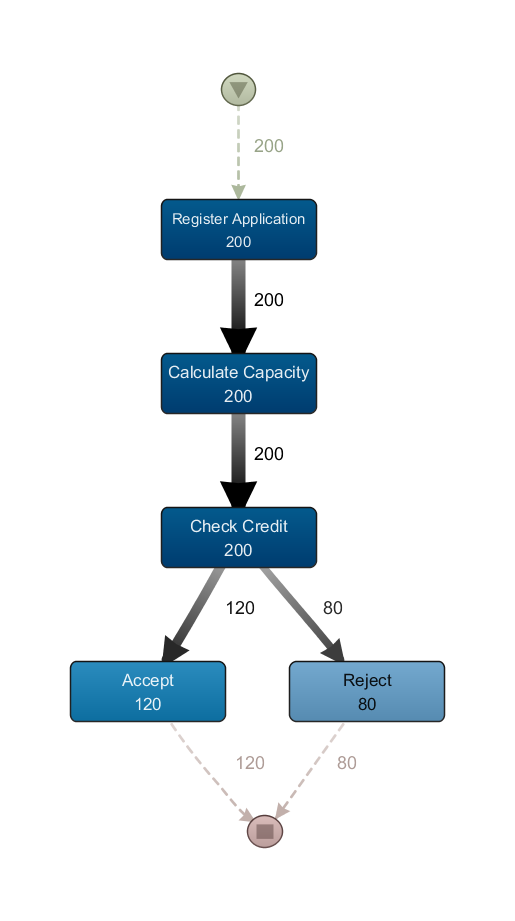
\includegraphics[width=.8\linewidth]{5_results_discussions/loan-application-process/ETM_Configuration3}
    \caption{Variant \#3}
    \label{fig:loan-application-process-models-3}
  \end{subfigure}%
  \begin{subfigure}{.4\textwidth}
    \centering
    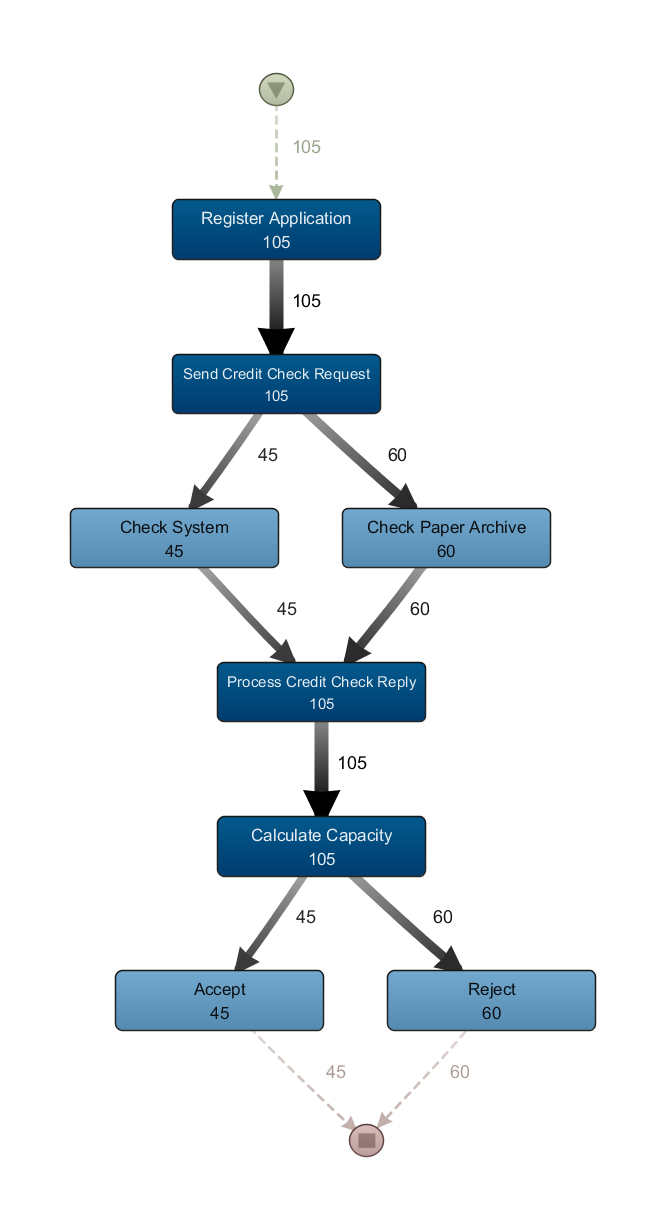
\includegraphics[width=.8\linewidth]{5_results_discussions/loan-application-process/ETM_Configuration4}
    \caption{Variant \#4}
    \label{fig:loan-application-process-models-4}
  \end{subfigure}
\caption{Process models of Loan Application Process dataset}
\label{fig:loan-application-process-models}
\end{figure} 

In \textit{Performance Indicator Analysis} stage, firstly event logs are replayed over process models and performance indicators are calculated. For replaying step, alignment costs should be checked with respect to process model mining evaluation metrics; however, since all fitness values of variants are 100 \% in Table~\ref{table:loan-app-process-process-model-mining}, corresponding alignment costs are 0 for this dataset. This ensures that event logs are successfully replayed over process models and performance indicators are calculated. With these performance indicators, organizations are clustered and internal evaluation of clusters are presented with different number of clusters in Figure~\ref{fig:loan-cluster-sse-plot}. As expected, within-SSE value decreases when number of clusters, \textit{k}, increases. Considering the effects of overfitting after the \textit{elbow} point in the plot, number of clusters is selected to be 2 for this dataset. For two clusters, Variant \#1, \#2, and \#4 are grouped into one cluster where only Variant \#3 is left to other cluster.
\begin{figure}
	\centering
	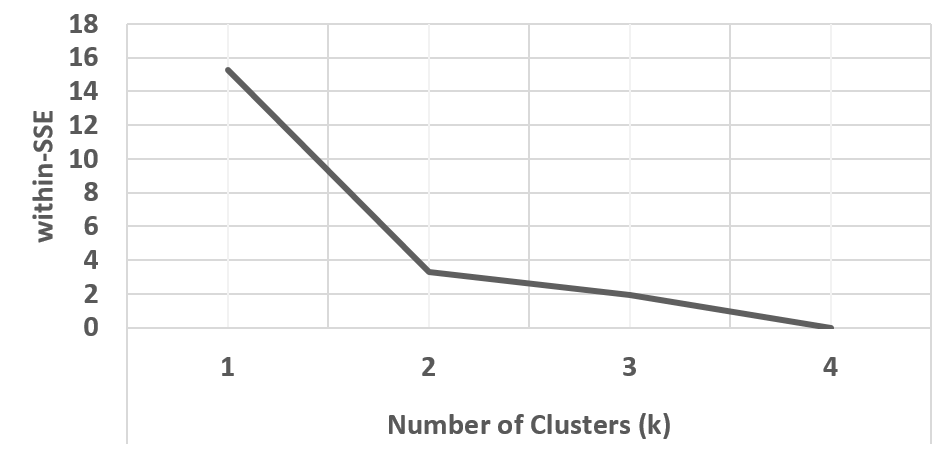
\includegraphics[width=.7\textwidth]{5_results_discussions/loan-application-process/cluster-sse-plot}
	\caption{Number of Clusters vs. within-SSE for Loan Application Process dataset}
  \label{fig:loan-cluster-sse-plot}
\end{figure}

In \textit{Mismatch Pattern Analysis} stage, number of mismatch patterns are analyzed with the \textit{graph-edit similarity} between each two organization. For each two organization, their \textit{graph-edit similarity} values are calculated and then our mismatch pattern analyzers are executed to spot differences. As the similarity between process models decreases our method spots more mismatch patterns for most of the variants and it ensures that the developed mismatch pattern analyzers work as expected for this dataset. Correlation between \textit{graph-edit similarity} and number of mismatch patterns are plotted in Figure~\ref{fig:loan-mismatch-pattern-analysis-results}.
\begin{figure}
	\centering
	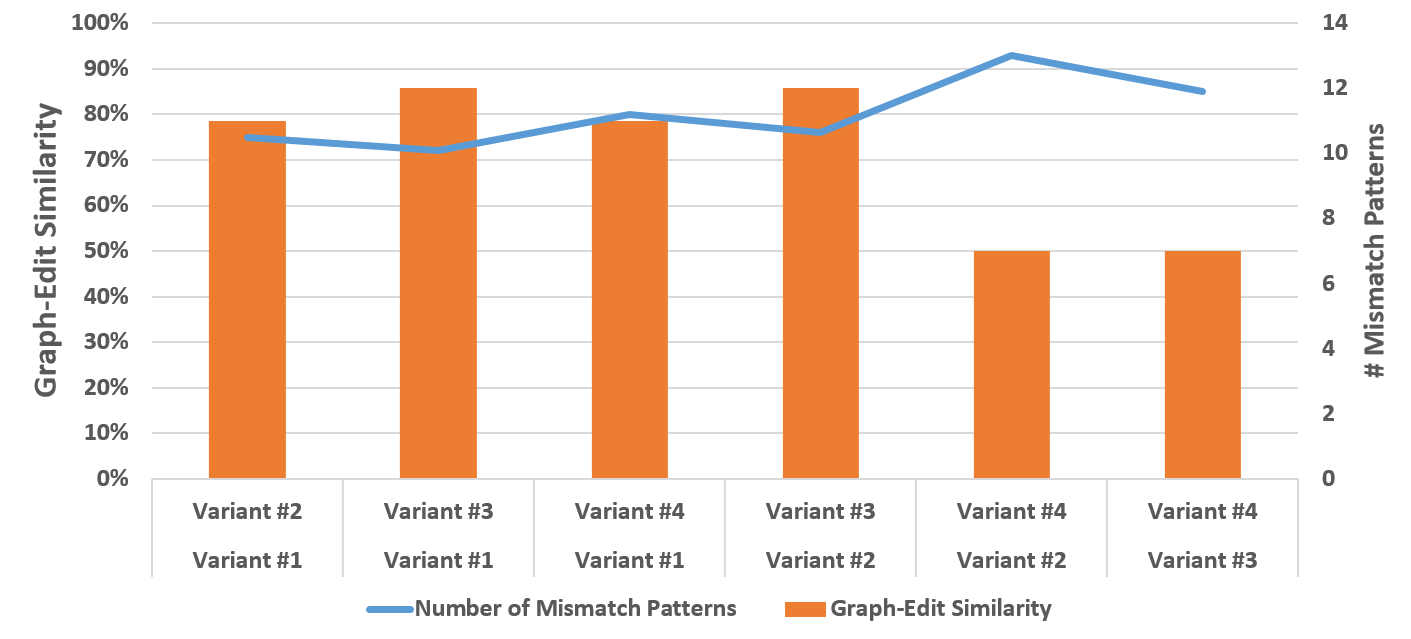
\includegraphics[width=\textwidth]{5_results_discussions/loan-application-process/mismatch-pattern-analysis-results}
	\caption{Mismatch Patterns vs. Graph-Edit Similarity for Loan Application Process variants}
  \label{fig:loan-mismatch-pattern-analysis-results}
\end{figure}

When the mismatch patterns are analyzed according to their types as diagrammed in Figure~\ref{fig:loan-mismatch-pattern-types}, \textit{"Skipped Activity"} and \textit{"Activities at Different Moments"} patterns are spotted mostly and no \textit{"Different Conditions for Occurrence"} or \textit{"Additional Dependencies"} patterns are discovered. Considering the small amount of this dataset, these numbers and distribution can be counted as acceptable in this stage of methodology.
\begin{figure}
	\centering
	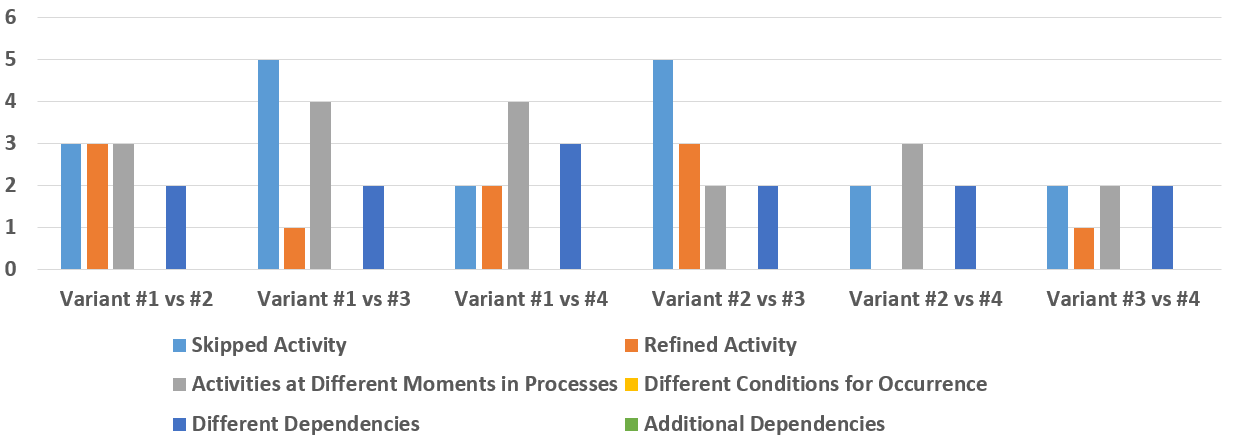
\includegraphics[width=\textwidth]{5_results_discussions/loan-application-process/mismatch-pattern-types}
	\caption{Mismatch pattern types for Loan Application Process variants}
  \label{fig:loan-mismatch-pattern-types}
\end{figure}
 
In \textit{Recommendation Generation} stage, an organization and performance difference threshold is selected as analysis input. For the selected organization's cluster, all other clusters are checked for performing better than the specified threshold. Instead of all mismatch patterns between organizations, only the mismatch patterns that are potential causes of other organizations to perform better are listed. For different threshold values, number of performance indicators that are performing better for the selected organization and spotted mismatch patterns are plotted in Figure~\ref{fig:loan-recommendation-generation-analysis}. 
\begin{figure}
	\centering
	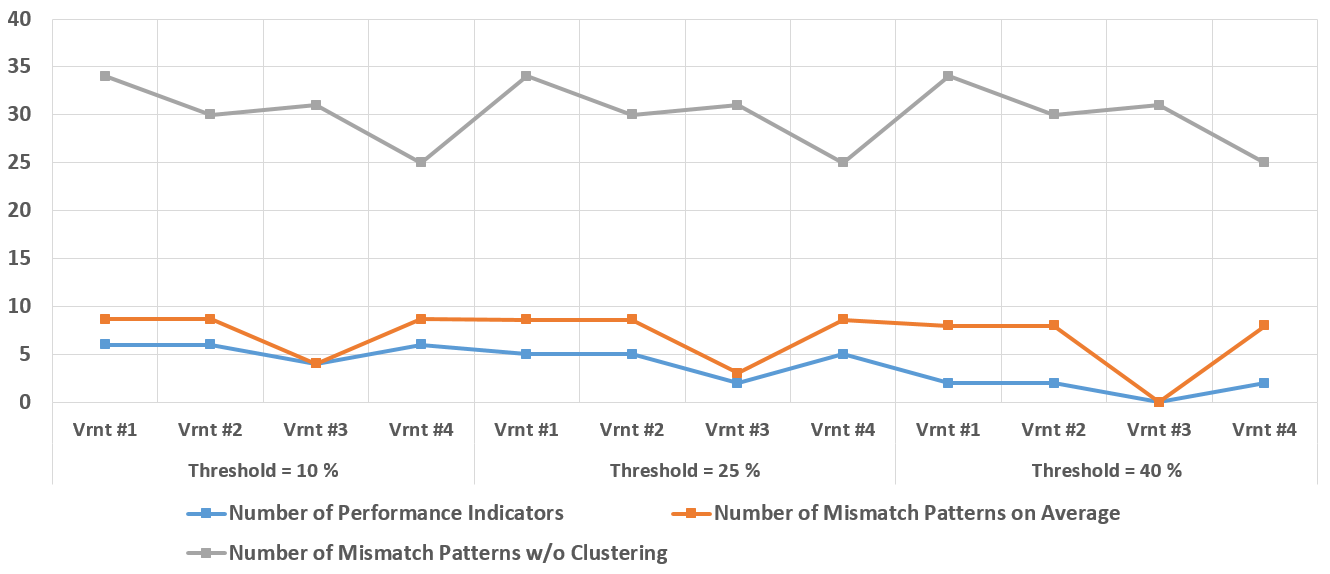
\includegraphics[width=\textwidth]{5_results_discussions/loan-application-process/recommendation-generation-analysis}
	\caption{Recommendation Generation analysis for Loan Application Process dataset}
  \label{fig:loan-recommendation-generation-analysis}
\end{figure}

In order to construct the data in Figure~\ref{fig:loan-recommendation-generation-analysis}, every organization is selected one-by-one with different threshold values. For every analysis, number of performance indicators and average number of mismatch patterns causing them are plotted. In addition, total number of mismatch patterns without clustering for each organization is added to the plot as an upper bound. With the help of this upper bound, responsiveness and degree of helping the user to focus on the performance improvement can be analyzed. As can be seen, for each threshold value, average number of mismatch patterns \textit{with performance indicator clustering} are very low compared to \textit{without clustering}. In other words, when user wants to improve its performance with any threshold, there is significantly less number of mismatch patterns on average to check. This shows the methodology proposed in this thesis can help users to focus on differences between organizations given this dataset. 